\documentclass{beamer}

\mode<presentation>
{
  \usetheme{Darmstadt}
  \usecolortheme{default}
  \usefonttheme{default}
  \setbeamertemplate{navigation symbols}{}
  \setbeamertemplate{caption}[numbered]
}

\usepackage[english]{babel}
\usepackage[utf8x]{inputenc}
\usepackage{listings}

\lstdefinestyle{customc}{
  belowcaptionskip=1\baselineskip,
  breaklines=true,
  xleftmargin=\parindent,
  language=C,
  showstringspaces=false,
  basicstyle=\footnotesize\ttfamily,
  keywordstyle=\bfseries\color{green!40!black},
  commentstyle=\itshape\color{purple!40!black},
  identifierstyle=\color{blue},
  stringstyle=\color{orange},
  basicstyle=\ttfamily\scriptsize,
  columns=fullflexible,
}

\title{libxively internals}
\subtitle{A not-so-gentle introduction}
\author{Olgierd Humeńczuk}
\date{\today}

\begin{document}

\begin{frame}
	\titlepage
\end{frame}

\begin{frame}{Brief Outline}
	\tableofcontents
\end{frame}

\section{Introduction}

\subsection{Motivation}

\begin{frame}{Design goals}

\begin{itemize}[<+->]
    \item Simple to use API
    \item Must work with different OS's
    \item Must work even with no OS on MCUs
    \item Robust
    \item Small power consumption $=$ high efficiency
    \item Smallest possible memory consumption $\neq$ high efficiency
    \item Modern
\end{itemize}

\end{frame}

\subsection{Techniques used}

\begin{frame}{Programming Concepts}

\begin{itemize}[<+->]
    \item Asynchronicity
    \item Continuations
    \begin{itemize}[<+->]
        \item Protothreads\footnote{\url{http://dunkels.com/adam/pt/}}
    \end{itemize}
    \item Event-driven approach with reactor pattern inspired by
    \begin{itemize}[<+->]
        \item \texttt{boost::asio}
        \item Twisted Python
        \item Node.js
    \end{itemize}
\end{itemize}

\end{frame}

\section{Design}

\subsection{General Architecture Description}

\begin{frame}{Layers}

\begin{columns}
    \begin{column}{0.5\textwidth}
        \centerline{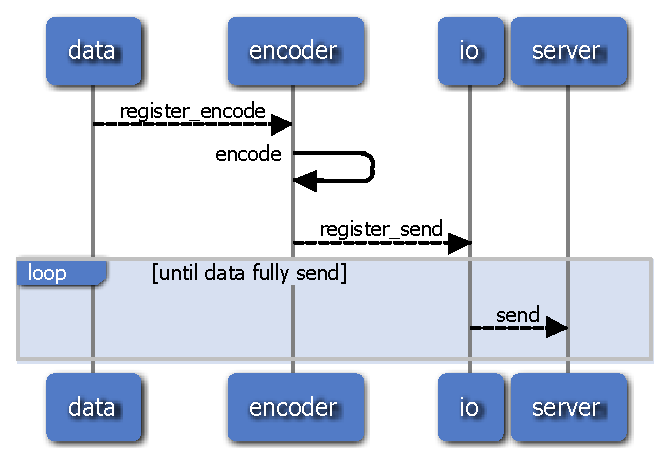
\includegraphics[width=1.0\textwidth]{design-intro.slides/layer.pdf}}
    \end{column}
    \pause
    \begin{column}{0.5\textwidth}
        \begin{itemize}[<+->]
            \item Layers design inspired by
                \begin{itemize}[<+->]
                    \item Twisted
                    \item Linux pipes
                \end{itemize}
            \item Separation of concerns
            \item Unified API
            \item Ability to add some encoders \& decoders later without changing all of the existing code
            \item Easy to stub-out for unit testing, all it's got is input \& output, just a black box
        \end{itemize}
    \end{column}
\end{columns}

\end{frame}

\begin{frame}{Continuations}
    \begin{columns}
        \begin{column}{0.5\textwidth}
            \centerline{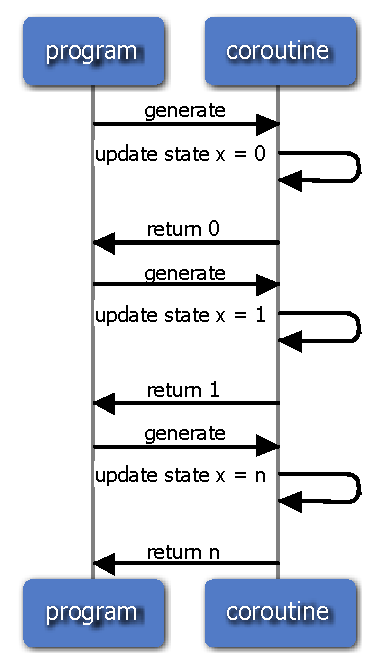
\includegraphics[width=0.75\textwidth]{design-intro.slides/coroutine_idea.pdf}}
        \end{column}
        \pause
        \begin{column}{0.5\textwidth}
            \begin{itemize}[<+->]
                \item Coroutines inspired by
                    \begin{itemize}[<+->]
                        \item Protothreads
                    \end{itemize}
                \item Hugely simplifies asynchronous code readability
                \item Hugely simplifies asynchronous code readability
                \item Hugely simplifies asynchronous code readability
                \item Great for lazy generators
                \item Great for splitting-up complex control flow
            \end{itemize}
        \end{column}
    \end{columns}
\end{frame}

\begin{frame}{Continuations a.k.a. Coroutines a.k.a. Micro Threads example}
    \lstinputlisting[style=customc]{design-intro.slides/coro.c}
\end{frame}

\begin{frame}{Event Dispatcher}
    \begin{columns}
        \begin{column}{0.5\textwidth}
            \centerline{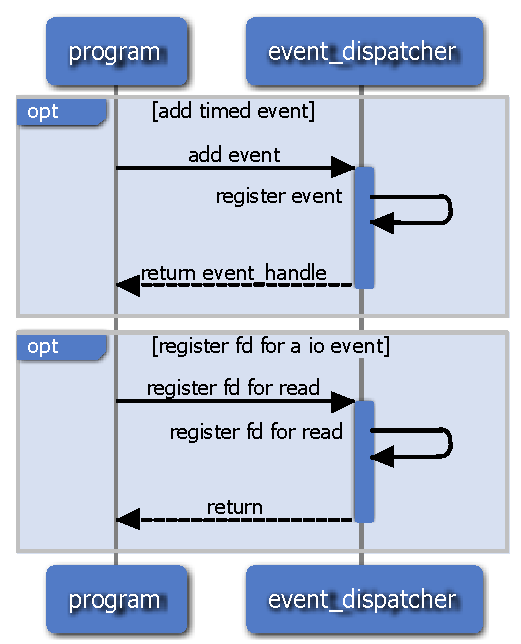
\includegraphics[width=0.75\textwidth]{design-intro.slides/evtd_basics.pdf}}
        \end{column}
        \pause
        \begin{column}{0.5\textwidth}
            \begin{itemize}[<+->]
                \item Event Dispatcher inspired by
                    \begin{itemize}[<+->]
                        \item \texttt{boost::asio}
                        \item Twisted Python
                    \end{itemize}
                \item Implements timers and I/O events
                \item Execution can wait passively
                \item Code is organised with callbacks
                \item Allows for stack-less code design
            \end{itemize}
        \end{column}
    \end{columns}
\end{frame}

\section{Examples}

\subsection{Use Cases}

\begin{frame}{Simple timed event}
    \centerline{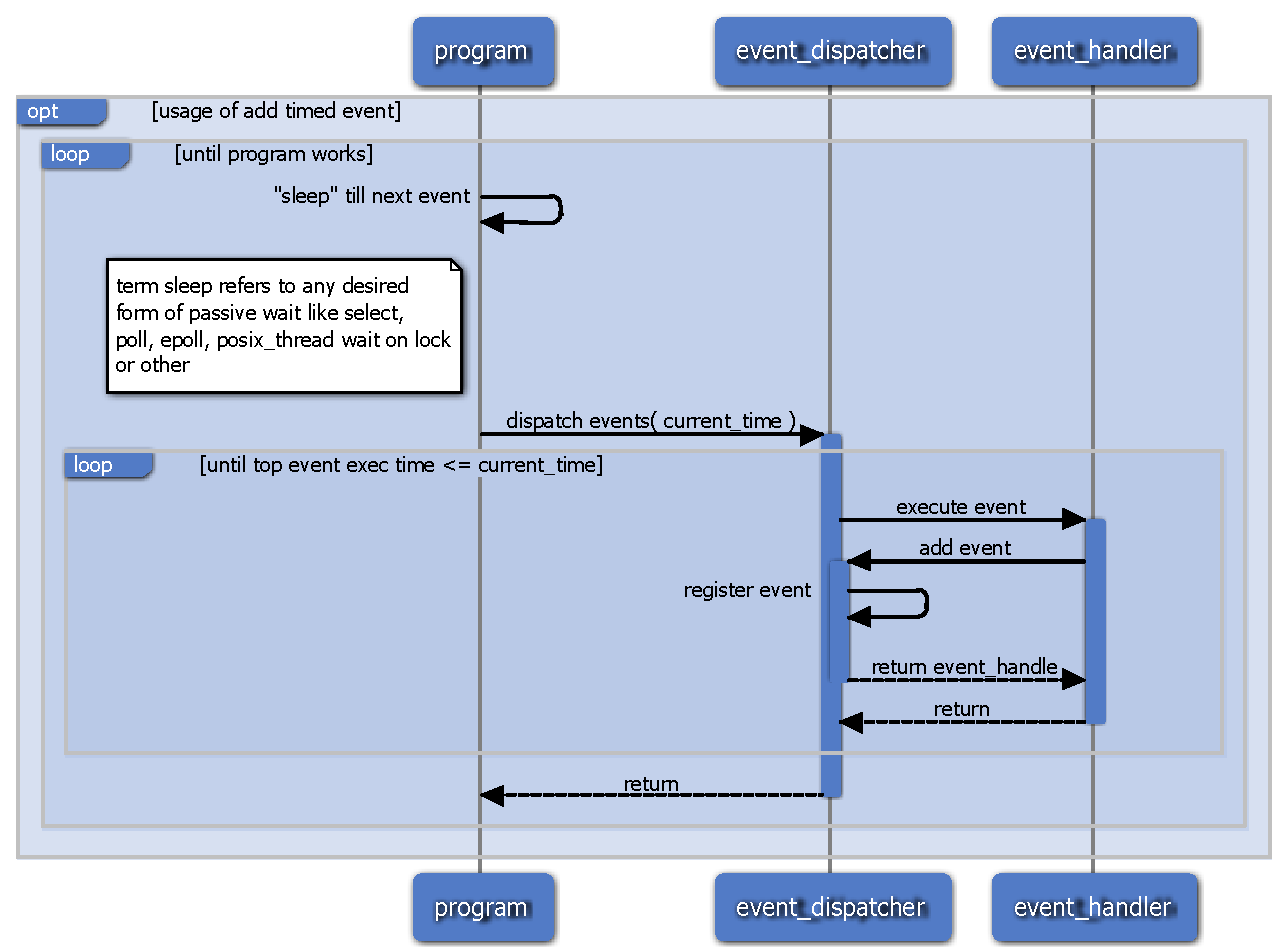
\includegraphics[width=0.88\textwidth]{design-intro.slides/evtd_details_time.pdf}}
\end{frame}

\begin{frame}{Sending data to the server}
    \centerline{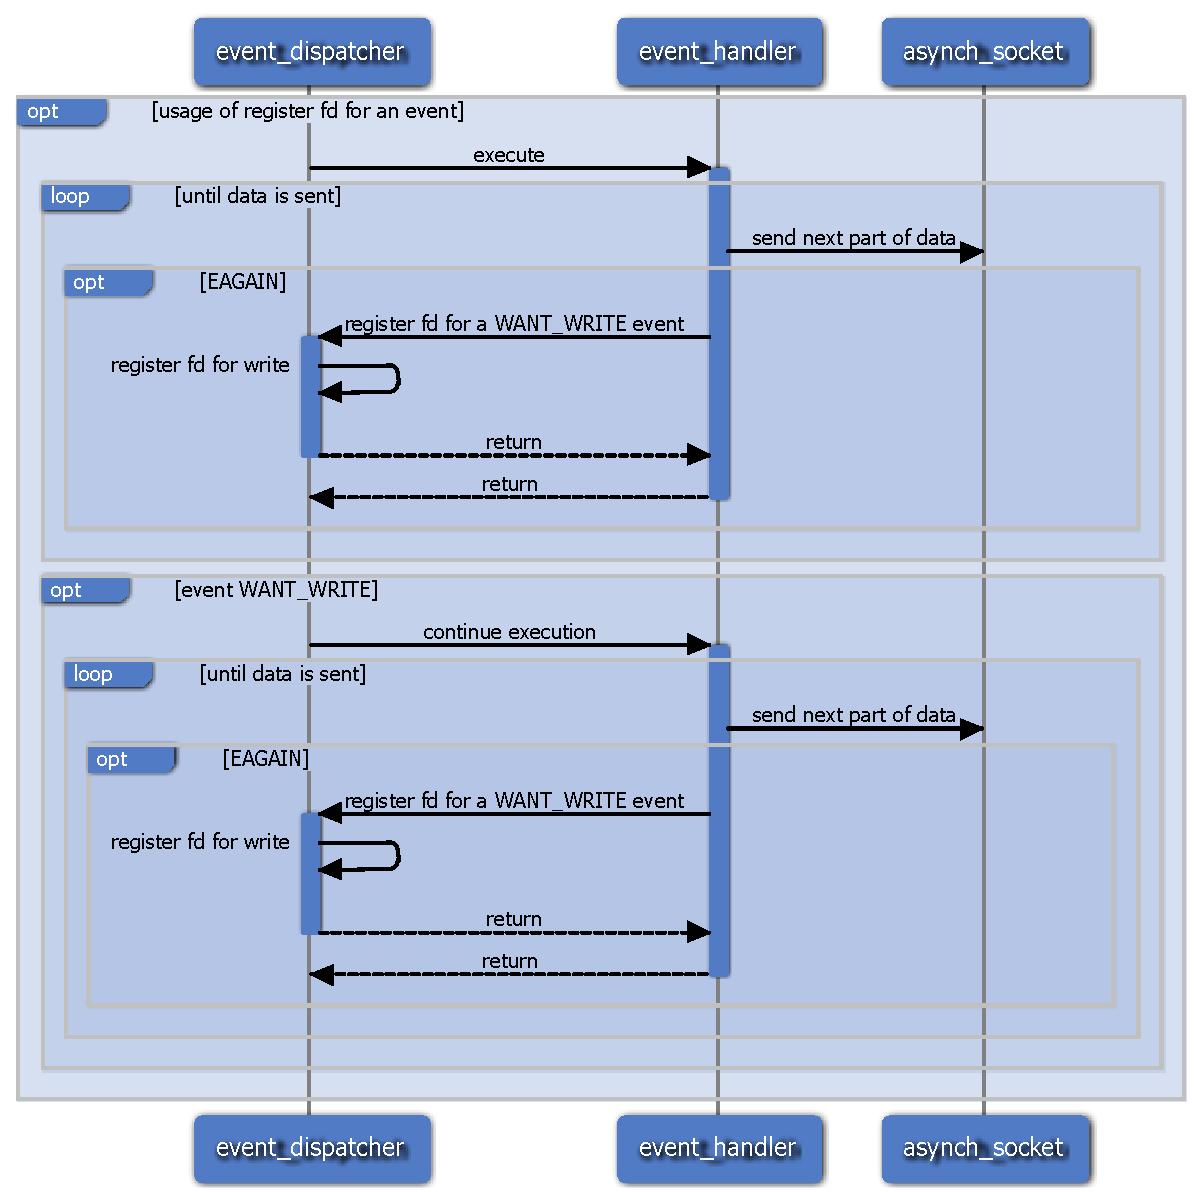
\includegraphics[width=0.70\textwidth]{design-intro.slides/evtd_details_send.pdf}}
\end{frame}

\subsection{MQTT}

\begin{frame}{MQTT send}
    \centerline{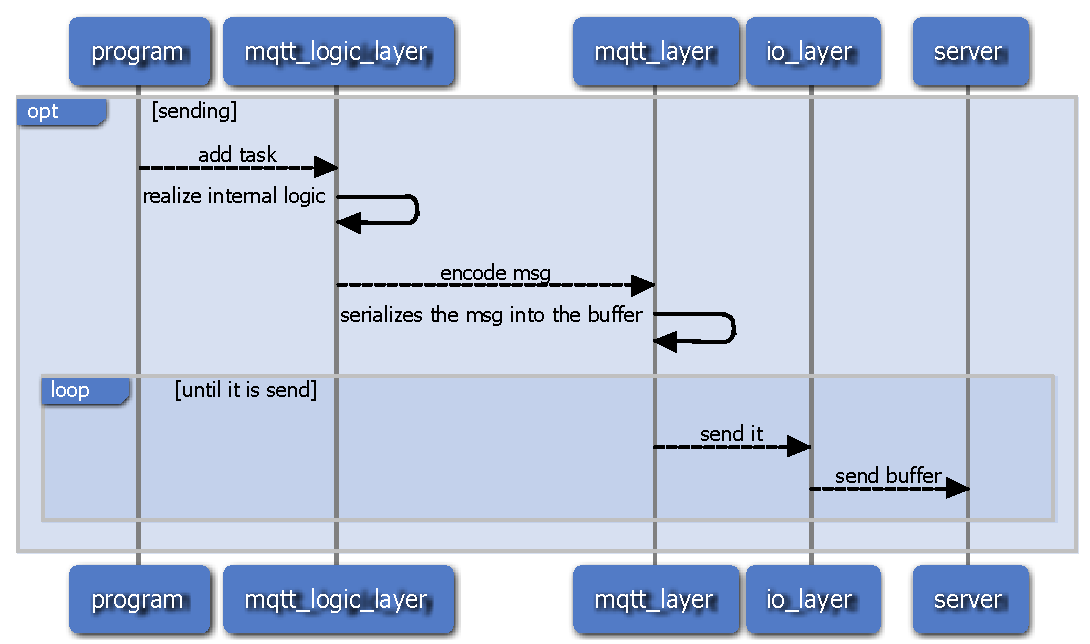
\includegraphics[width=0.75\textwidth]{design-intro.slides/mqtt_send.pdf}}
\end{frame}

\begin{frame}{MQTT receive}
    \centerline{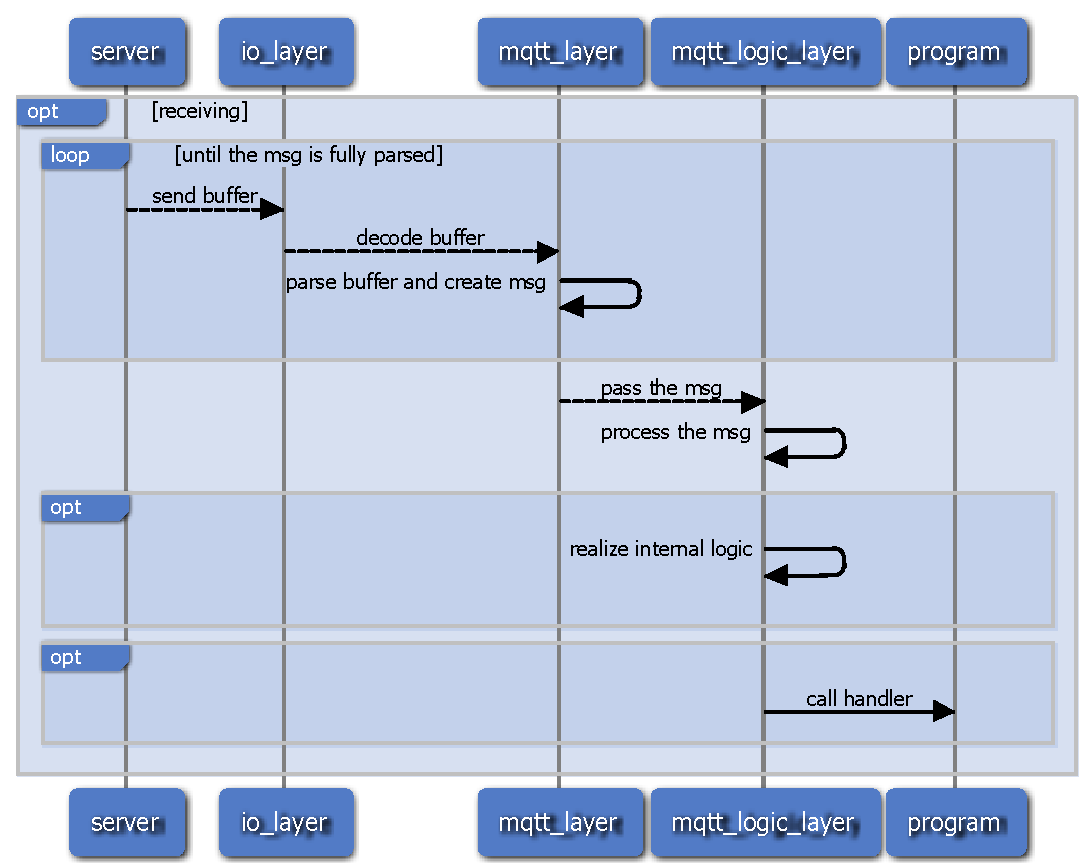
\includegraphics[width=0.75\textwidth]{design-intro.slides/mqtt_recv.pdf}}
\end{frame}

\section{The End}

\subsection{Thank you!}

\begin{frame}{Q\&A}
Questions or comments?
\end{frame}

\end{document}
